% !TeX root = ../main.tex

\chapter{Examples of Figures and Tables}

\section{Figures}

Figures are normally inserted in \env{figure} environments by \cs{includegraphics}
You can refer to the source code of Figure~\ref{fig:example}.

It is recommended to use PDF format for vector figures, and JPG format for bitmaps. TIFF format is not supported.

\begin{figure}
  \centering
  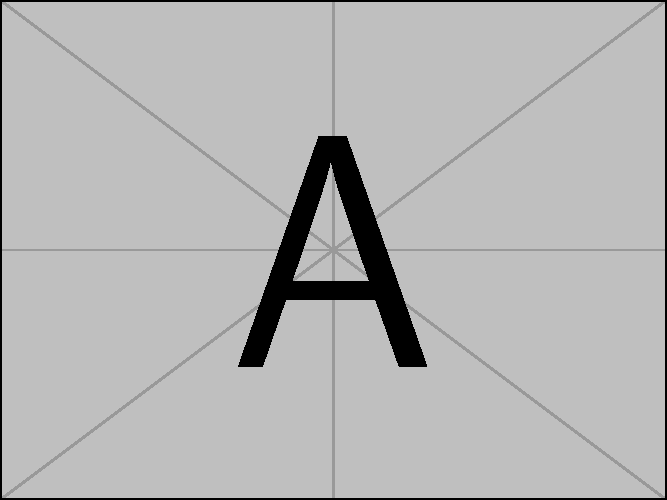
\includegraphics[width=0.6\linewidth]{example-image-a.pdf}
  \caption{Example figure.}
  \label{fig:example}
\end{figure}

If a figure is consisted of two or more sub-figures, the sub-figures should be numbered in (a), (b), (c), etc. and should have sub-captions.

\begin{figure}
  \centering
  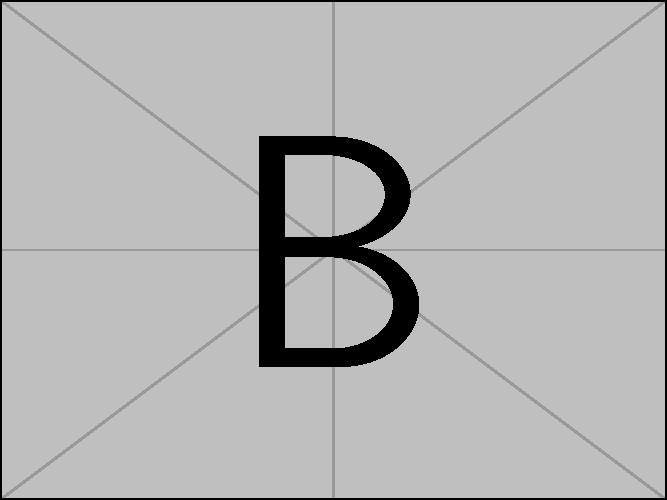
\includegraphics[width=0.6\linewidth]{example-image-b.pdf}
  \caption{Example figure b.}
  \label{fig:example-b}
\end{figure}

It is recommended to use \pkg{subcaption} package to deal with sub-figures, such as Figure~\ref{fig:subfig-a} and Figure~\ref{fig:subfig-b}.

\begin{figure}
  \centering
  \subcaptionbox{Sub-figure A\label{fig:subfig-a}}
    {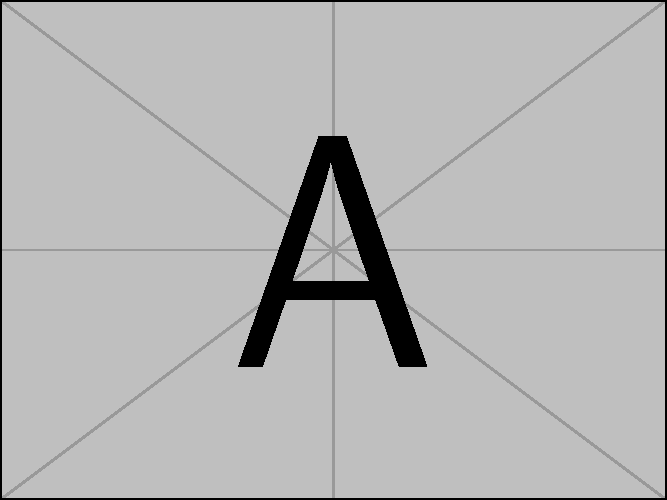
\includegraphics[width=0.45\linewidth]{example-image-a.pdf}}
  \subcaptionbox{Sub-figure B\label{fig:subfig-b}}
    {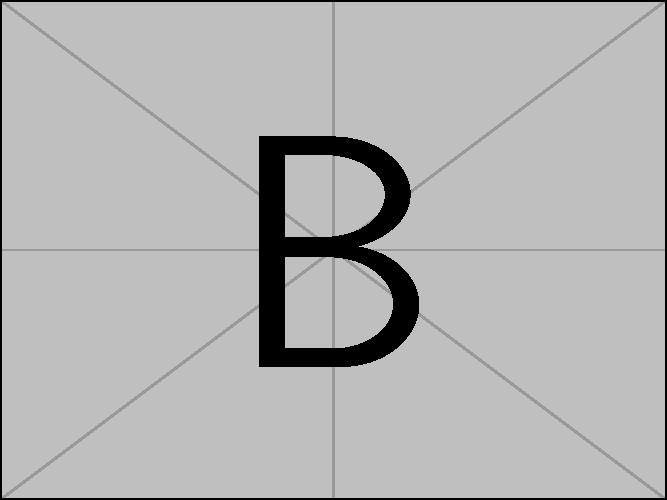
\includegraphics[width=0.45\linewidth]{example-image-b.pdf}}
  \caption{Example figure with two sub-figures.}
  \label{fig:multi-image}
\end{figure}



\section{Tables}

Tables should be self-explanatory. Three line tables are recommended for clearance, such as Table~\ref{tab:three-line}. The three lines can be generated by commands provided by \pkg{booktabs}.

\begin{table}
  \centering
  \caption{Example of a three line table}
  \begin{tabular}{ll}
    \toprule
    Filename          & Description                         \\
    \midrule
    thuthesis.dtx   & 模板的源文件,包括文档和注释 \\
    thuthesis.cls   & 模板文件                     \\
    thuthesis-*.bst & BibTeX 参考文献表样式文件    \\
    thuthesis-*.bbx & BibLaTeX 参考文献表样式文件  \\
    thuthesis-*.cbx & BibLaTeX 引用样式文件        \\
    \bottomrule
  \end{tabular}
  \label{tab:three-line}
\end{table}

If you need to include notes in tables, the package \pkg{threeparttable} can be used.
You must use lower-case letters (a, b, c, ...) to number the notes.

\begin{table}
  \centering
  \begin{threeparttable}[c]
    \caption{Example of a table with notes}
    \label{tab:three-part-table}
    \begin{tabular}{ll}
      \toprule
      Filename                 & Description                         \\
      \midrule
      thuthesis.dtx\tnote{a} & 模板的源文件,包括文档和注释 \\
      thuthesis.cls\tnote{b} & 模板文件                     \\
      thuthesis-*.bst        & BibTeX 参考文献表样式文件    \\
      thuthesis-*.bbx        & BibLaTeX 参考文献表样式文件  \\
      thuthesis-*.cbx        & BibLaTeX 引用样式文件        \\
      \bottomrule
    \end{tabular}
    \begin{tablenotes}
      \item [a] 可以通过 xelatex 编译生成模板的使用说明文档;
        使用 xetex 编译 \file{thuthesis.ins} 时则会从 \file{.dtx} 中去除掉文档和注释,得到精简的 \file{.cls} 文件。
      \item [b] 更新模板时,一定要记得编译生成 \file{.cls} 文件,否则编译论文时载入的依然是旧版的模板。
    \end{tablenotes}
  \end{threeparttable}
\end{table}

The package \pkg{longtable} can be used for cross-page tables.
The number of the table should be repeated on each page, followed by the caption of the table and ``(continued)''. Table heads must also be repeated on continued tables.

\begin{longtable}{cccc}
    \caption{Example of a cross-page long table.} \\
    \toprule
    Column 1 & Column 2 & Column 3 & Column 4 \\
    \midrule
  \endfirsthead
    \caption[]{Example of a cross-page long table (continued).} \\
    \toprule
    Column 1 & Column 2 & Column 3 & Column 4 \\
    \midrule
  \endhead
    \bottomrule
  \endfoot
  Row 1  & & & \\
  Row 2  & & & \\
  Row 3  & & & \\
  Row 4  & & & \\
  Row 5  & & & \\
  Row 6  & & & \\
  Row 7  & & & \\
  Row 8  & & & \\
  Row 9  & & & \\
  Row 10 & & & \\
  Row 11 & & & \\
  Row 12 & & & \\
  Row 13 & & & \\
  Row 14 & & & \\
  Row 15 & & & \\
  Row 16 & & & \\
  Row 17 & & & \\
  Row 18 & & & \\
  Row 19 & & & \\
  Row 20 & & & \\
  Row 21 & & & \\
  Row 22 & & & \\
  Row 23 & & & \\
  Row 24 & & & \\
  Row 25 & & & \\
  Row 26 & & & \\
  Row 27 & & & \\
  Row 28 & & & \\
  Row 29 & & & \\
  Row 30 & & & \\
  Row 31 & & & \\
  Row 32 & & & \\
  Row 33 & & & \\
  Row 34 & & & \\
  Row 35 & & & \\
  Row 36 & & & \\
  Row 37 & & & \\
  Row 38 & & & \\
  Row 39 & & & \\
  Row 40 & & & \\
\end{longtable}
